\documentclass[10pt]{beamer}
\usetheme{Boadilla}
%\setbeamersize{text margin left=30mm,text margin right=30mm} 

% \usepackage{times}
\usepackage[sfdefault]{FiraSans} %% option 'sfdefault' activates Fira Sans as the default text font
\usepackage[T1]{fontenc}

\usepackage[square,numbers]{natbib}
\usepackage{graphicx}
\usepackage{xcolor}
\usepackage{geometry}
\usepackage{hyperref}
\usepackage[margin=0.8cm]{caption}
\usepackage{amsmath}
\usepackage{booktabs} % Allows the use of \toprule, \midrule and \bottomrule in tables
\usepackage{subcaption}

% Font sizes
\newcommand\Fontvi{\fontsize{6}{7.2}\selectfont}
\newcommand\Fontvii{\fontsize{7}{8.4}\selectfont}
\newcommand\Fontviii{\fontsize{8}{9.6}\selectfont}
\newcommand\Fontix{\fontsize{9}{10.8}\selectfont}
\newcommand\Fontx{\fontsize{10}{12.0}\selectfont}
\newcommand\Fontxi{\fontsize{11}{13.2}\selectfont}

\newcommand\sun{\hbox{$\odot$}}
\newcommand\earth{\hbox{$\oplus$}}
\newcommand\degr{\hbox{$^\circ$}}
\newcommand\arcmin{\hbox{$^\prime$}}
\newcommand\arcsec{\hbox{$^{\prime\prime}$}}

\newcommand\micron{\hbox{$\umu$m}}
\newcommand\ion[2]{\text{#1\,\textsc{\lowercase{#2}}}}  % ionization states

\title[Short title]{A long title - whats that about?}
\subtitle{{\color{gray} \small An even longer subtitle to take even longer time to read.}}
\author[Soumyadeep Das]{Soumyadeep Das}
\institute[Uni of Hertfordshire]{Centre for Astrophysics Research (CAR)\\University of Hertfordshire\\Hatfield (United Kingdom).}
\date{}

\begin{document}
{
\usebackgroundtemplate{\includegraphics[width=\paperwidth]{back.pdf}}
  
  \begin{frame}
    \titlepage
  \end{frame}
}

% \begin{frame}
% \frametitle{Outline}
% \tableofcontents
% \end{frame}

\section{Overview of this Project}
\begin{frame}
\frametitle{Overview of this Project}
\Fontvii
\begin{columns}[T] % align columns
\begin{column}{.40\textwidth}
\begin{itemize}
  \item Brightest Cluster Galaxy of Abell 569.
  \item Two pairs of misaligned radio lobes at different scales : 100 kpc WAT FRI lobes and the 10 kpc bubble-like Seyfert lobes.
  \item One-sided core-jet VLBI structure, jet aligned along NW FRI lobe.
  \item Host galaxy ambiguous -  Either elliptical/bulge-dominated or lenticular (S0).
  \item Small optical jet-like extension aligned along the VLBI jet.
  \vspace*{0.2cm}
  {\color{gray} \hrule}
  \vspace*{0.1cm}
  \item Imaged archival VLA and VLBA data at all available frequencies and scales - using AIPS and CASA. 
  \item Obtained spectral index images and calculated equipartition parameters and age estimates.
  \item Also looked at optical HST images and X-ray images from Chandra and Einstein.
\end{itemize}
\end{column}%
\hfill%
\begin{column}{.59\textwidth}
\begin{figure}[htbp]
\vspace*{-1cm}
\centering
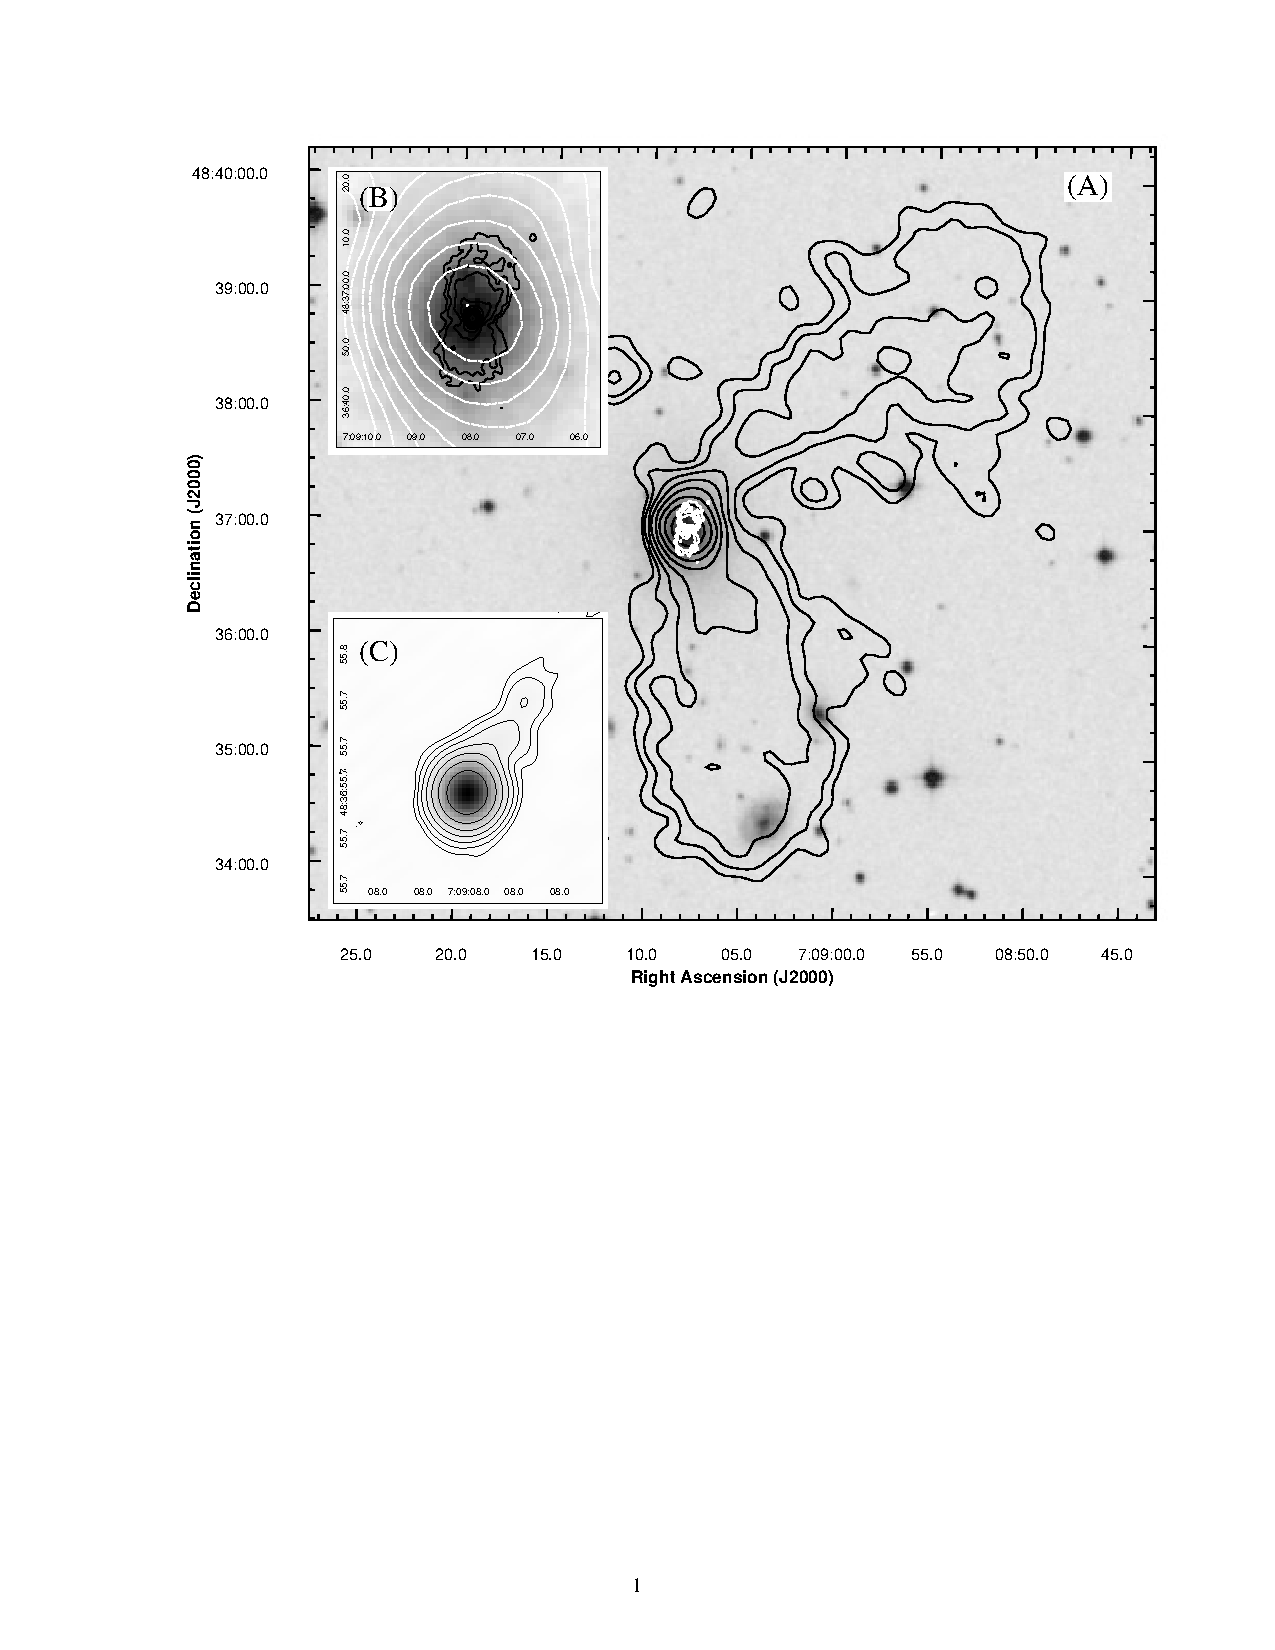
\includegraphics[trim=2.8cm 10.4cm 1.6cm 2.0cm,clip,width=6.5cm]{combined.pdf}
\caption*{\Fontvi \centering VLA radio contour images of NGC\,2329 at different scales overlaid on the DSS POSS2 optical image. (A) 1.4~GHz 16$\arcsec$ VLA contours are in black, and 1.4~GHz 1$\arcsec$ VLA contours in white. (B) Zoomed in snapshot of the inner Seyfert lobes in black. (C) 4.99~GHz 4~mas VLBA radio contour image.}
\end{figure} 
\end{column}%
\end{columns}
\end{frame}


% HERE
\begin{frame}
\frametitle{\large VLA Total Intensity \& Spectral Index Images}
\Fontviii
\begin{itemize}
  \item FRI lobes are much dimmer than the Seyfert lobes.
  \item FRI lobes are not edge-brightened and devoid of compact features like jet knots.
  \item Mean spectral index ($\alpha^{1.4}_{4.7})$ values-\\Seyfert lobes  : $-0.75\pm0.16$\\NW FRI lobes : $-1.31\pm0.18$\\South FRI lobes  : $-1.04\pm0.13$.
  \item Spectral index across the FRI lobes in NGC 2329 is almost uniform without signs of any significant steepening.
  \item VLBI jet speed $\sim 0.75c$ - similar to FRI sources.
\end{itemize}
\end{frame}
% TO HERE

\begin{frame}
\Fontviii
\frametitle{Acknowledgments}
\hspace*{0.5cm}
\begin{itemize}
  \item The Project `The Peculiar WAT NGC 2329 - Case for AGN Restart?' was conducted under the Visiting Student's Research Programme (NCRA-TIFR) and supervised Dr Preeti Kharb, NCRA-TIFR, India. Further works were done in collaboration with Prof Raffaella Morganti, ASTRON, and Dr Sumana Nandi, NCRA-TIFR.
  \hspace*{0.5cm}
  \item Sikora, M., Stawarz, L., \& Lasota, J. (2007). Radio Loudness of Active Galactic Nuclei: Observational Facts and Theoretical Implications. The Astrophysical Journal, 658(2), 815–828. https://doi.org/10.1086/511972    
\end{itemize}
\hspace*{0.5cm}
I sincerely thank Dr Christopher Harrison, Dr Danielle Leonard, and Newcastle University for this interview.
\end{frame}

\end{document}


